%TODO Add forkId (version of the zkEVM)

\section{Introduction}

This document specifies how the polygon zkEVM is proven using 
recursion, agregation and composition.
The constraints of the zkEVM are specified as polynomial identities using the 
PIL language. Then, an execution trace can be proven using the PIL specification for 
building a STARK that is proved with the FRI protocol.
The problem is that STARKs generate big proofs. 
This document describes how to use recursion together with composition to shorten the prove size.

In a high level, a basic recursion block transforms a PIL specification into the 
specification of its STARK verification circuit (written in Circom). 
The circuit verifies the STARK of the PIL specification. 
Then, the Circom specification is transformed into a Plonkish PIL specification and the process is iterated.

In addition to recursion, also aggregation is implemented so that provers 
can aggregate the proofs of multiple transaction batches. 


\ifBACKGROUND
\section{Background}

%%%%%%%%%%%%%%%%%%%%%%%%%%%%%%%%%%%%%%%%%%%%%%%%%%%%%%%%%%%%%%%%%%%
\subsection{SNARK Composition} \label{sec:composition}

Imagine that we have two SNARK proof systems, $\A$ and $\B$, with different cost profiles. For example, assume that the prover in the first $\A$ is very fast, but the proof size is too large and the verification time is so slow to be directly deployed in practise. In contrast, the prover is second $\B$ is really slow, but the proof size is short and the verification time as good as it can be. Even if this looks like a very artificial scenario, this actually happens very often in the real world; where different state-of-the-art SNARKs have different trade-offs and therefore one has to choose the best one, in terms of costs, for his specific use case.

The previous situation depicts the following question: is it possible to combine them in some way to obtain a SNARK that inherits the best costs of both $\A$ and $\B$? More specifically, we want to obtain a SNARK $\C$ with the fast prover of $\A$ and the short proof size and fast verification time of $\B$.

Theoretically, it is possible via \textit{proof composition} which works as follows. Denote by $(\P_X, \V_X)$ the prover and the verifier of some SNARK $X$.  Say that $\P_{\C}$ claims to know a witness for a particular statement. First, $\P_{\C}$ uses $\P_{\A}$ to generate a SNARK proof $\pi$ of the claim. However, since $\pi$ is big and slow to verify, $\P_{\C}$ does not directly send $\pi$ to $\P_{\C}$. Instead, $\P_{\C}$ uses $\B$ to generate a proof $\pi'$ for the following statement:
\begin{center}
	``I know a proof $\pi$ for the original statement that makes $\V_{\A}$ accept with high probability.''
\end{center}
Then, $\P_{\C}$ sends $\pi'$ to $\V_{\C}$. In other words, $\P_{\C}$ uses $\P_{\A}$ to generate a proof $\pi$, then writes down the verification procedure of $\V_{\A}$ as a statement, uses $\P_{\B}$ to generate the proof $\pi'$ and finally uses $\V_{\B}$ to verify $\pi'$. Figure \ref{fig:composition} shows a diagram for this whole process.

It is important to remark here that proof composition requires taking the verification procedure as carried on by $\V_{\A}$ and written down in the underneath computational model used by $\B$. Hence, if arithmetic circuits are used, then one must write the verification part as an arithmetic circuit satisfiability instance.

\begin{figure}[H]
	\centering
	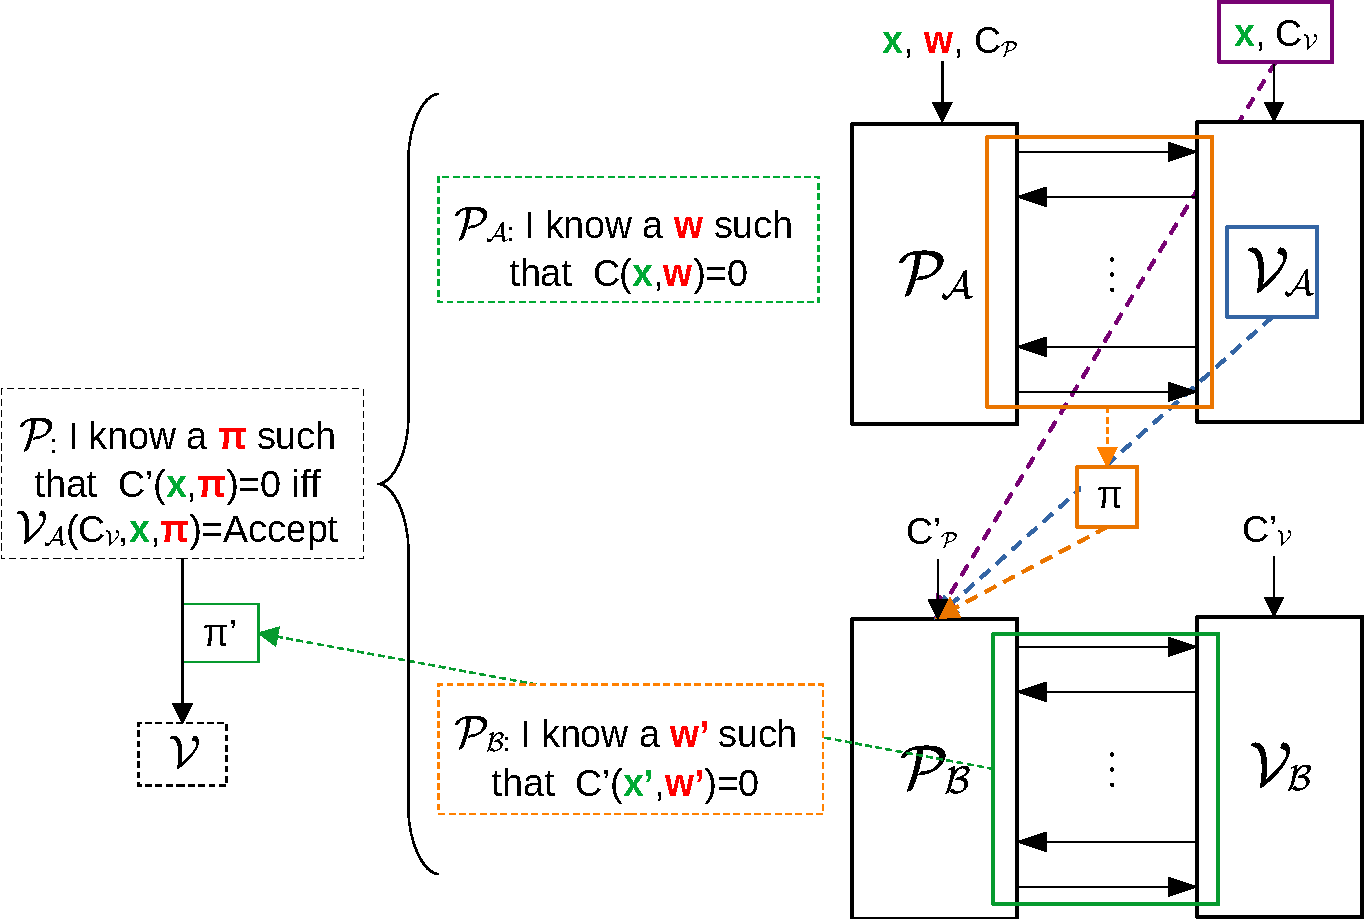
\includegraphics[width=.75\textwidth]{\recursiondir/figures/composition-diagram}
	\caption{Resulting statement obtained from a (depth-$1$) SNARK composition.}
	\label{fig:composition}
\end{figure}

\paragraph*{Costs of the Composition.}
Let's now discuss the costs of $\C$. Since $\P_{\C}$ only sends the second proof $\pi'$ to $\V_{\C}$, the proof size of $\C$ is the size of $\pi'$ as generated by $\V_{\B}$. Moreover, the verification time is precisely the time that $\V_{\B}$ takes to verify $\pi'$. Since the proof size and verification time of $\B$ are short and fast, respectively, the proof size and verification time of $\C$ are short and fast as well.

On the other hand, $\P_{\C}$ first has to generate the proof $\pi$ using $\P_{\A}$, and then has to generate the proof $\pi'$ using $\P_{\B}$. As commented at the beginning of the section, $\P_{\A}$ is fast whereas $\P_{\B}$ is slow. Wouldn't this imply that $\P_{\C}$ is slow? The key point is that the circuit of the verification procedure of $\V_{\A}$ is much more small than the circuit used to compute the first proof, since the verification time taken by $\V_{\A}$ is small (even if not optimal). Hence, the time required by $\P_{\C}$ to generate the second proof $\pi'$ is tiny compared to the time required to compute $\pi$. So, the proving time of $\P_{\C}$ is almost equal to the proving time of $\P_{\A}$, which is fast by assumption.

The best costs of both SNARKs have been achieved.




%%%%%%%%%%%%%%%%%%%%%%%%%%%%%%%%%%%%%%%%%%%%%%%%%%%%%%%%%%%%%%%%%%%
\subsection{Deeper Composition and Proof Recursion}

In the previous section we have seen how SNARK composition looks like and explained it with the generic case of two distinct SNARKs. In this section we explore what happens when we compose a SNARK with itself many times. This procedure is known as \textit{proof recursion}, and its name originates from the resemblance of any computer program being able to be evaluated at itself.

Say that we have a SNARK $\A$ with both proof size and evaluation time of size $O\left(N^{1/2}\right)$. Composing $\A$ with itself yields a new SNARK with proof size and verification time $O\left(\left(N^{1/2}\right)^{1/2}\right) = O\left(N^{1/4}\right)$. One more invocation of $\A$ will yield a new SNARK with proof size and verification time $O\left(N^{1/8}\right)$. One might be attempted to think that this composition can be carried on as many times as he would like, so that proof size and verification time fits with his objectives. However, there exists some upper bound, known as the \textit{recursion threshold}, to the minimum size that can be reached. This threshold refers to the smallest circuit size $N^{\star}$ such that the verification procedure of the initial SNARK $\A$ cannot be represented by a circuit of size smaller than $N^{\star}$. One example of a recursion threshold is the one obtained by Halo \cite{EPRINT:BowGriHop19}, which was proven to be as big as $2^{17}$. Not surprisingly, if one reaches the threshold and instantiate $\A$ another time, not only the resulting SNARK does not reduce costs, but in fact increase them.

What happens with the proving time? Simply put: the more compositions the resulting SNARK is composed of, the more work the prover has to do. Recall from the previous section that the prover must compute one proof per instantiation of the SNARK. For example, if $\A$ is composed with itself three times, the computer first computes a proof $\pi$ that would convice the $\A$ verifier, then produce a proof $\pi'$ that it knows a valid $\pi$, and finally a proof $\pi''$ that it knows a valid $\pi'$. Ever if the consequent proofs take substantially less time than the first one, there is some more work to do that just producing $\pi$.





%%%%%%%%%%%%%%%%%%%%%%%%%%%%%%%%%%%%%%%%%%%%%%%%%%%%%%%%%%%%%%%%%%%
\subsection{Further Applications}

In the previous section we have seen that SNARK composition can be used to improve the overall efficiency of existing SNARKs. Even if complex, this is a generic strategy to improve state-of-the-art SNARKs to whom is unclear if some optimizations are possible, or even when such optimizations are constrained by theoretical bounds. Importantly, applications of proof composition are not restricted to be of efficiency nature. In this section we explore some more applications of proof composition.



\paragraph*{Iterative Computation.} An interesting application of proof recursion is the one of \textit{iterative computation}. In this context, a designated prover $\P$ intends to prove to a verifier $\V$ that for some (public or secret) input $x$ and a publicly known function $f$ we have that:
\[
	f^{(i)}(x) := \underbrace{f(f(\dots f(f}_{i}(x)) \dots)) = y,
\]
where $y$ is a public output. One might notice that applying the same function $f$ some amount of times to an input $x$ is the same as function composition. Hence, one can build SNARKs for iterative computation by generating a SNARK of a single iteration of $f$ on $x$ and then composing the SNARK with itself the requested number of times.

\paragraph*{Incrementally Verifiable Computation.} A generalization of iterative computation is \textit{incrementally verifiable computation}. The idea is that, after each iteration $i$ of $f$ on $x$, $\P$ is able to output a partial computation $y_i$ and a proof $\pi_i$ that $f^{(i)}(x) = y_i$. Then, possibly before performing another iteration, a verifier is able to check the proof $\pi_i$ and be sure with high probability that $f$ has been correctly applied up until this point. Moreover, any party can resume the computation from that point and still be able to generate subsequent proofs.

\paragraph*{Proof Aggregation.} \textit{Proof aggregation} is a particular type of proof composition in which multiple valid proofs can be all proven to be valid by comprising them all into one proof, called the \textit{aggregated proof}, and only validating the aggregated one. More formally, $T$ parties (possibly the same one) $\P_1, \dots, \P_T$ use some proof system to produce proofs $\pi_1, \dots, \pi_T$. Then, instead of having one verification procedure per each proof, composition is used to prove the following statement:
\begin{center}
	I know valid proofs $\pi_1, \dots, \pi_T$ such that $C(\pi_1, \dots, \pi_T) = 0$,
\end{center}
where $C$ is the arithmetic circuit representing the verification procedure of all $\pi_1, \dots, \pi_T$.

The notion of proof aggregation becomes useful in the context of distributed computation, where a computation is too heavy to be carried out by a single party. Instead, the party would break the computation in $T$ pieces and send each of these pieces to a different party, who would produce a proof along with the output of each part. Finally, the original party would combine all the pieces into the actual output and produce a proof of the whole computation.


\paragraph*{Application to Blockchain Scalability.} Some mentioned applications could be combined to achieve \textit{scalability of blockchains}. That is, in order for a blockchain to improve its throughput (i.e., number of transactions per second), which is typically limited by block size and block finding speed, one can choose to perform transactions off-chain and publish a proof of correct state evolution on-chain.

There are several ways of accomplishing the off-chain proof. One can go for computing a proof of a blockchain's state update due to transactions within a block and then simply verify the proof on-chain. Even if totally possible, this is not the lowest cost solution since a blockchain's scalability solution must consume as less storage and verification time as possible. Because of these objectives, a more appropriate proof management design can be obtained using proof composition and/or proof aggregation.
Figure \ref{fig:composition-blockchain} provides a possible proof-management design through a combination of both proof techniques.
\begin{figure}[H]
	\centering
	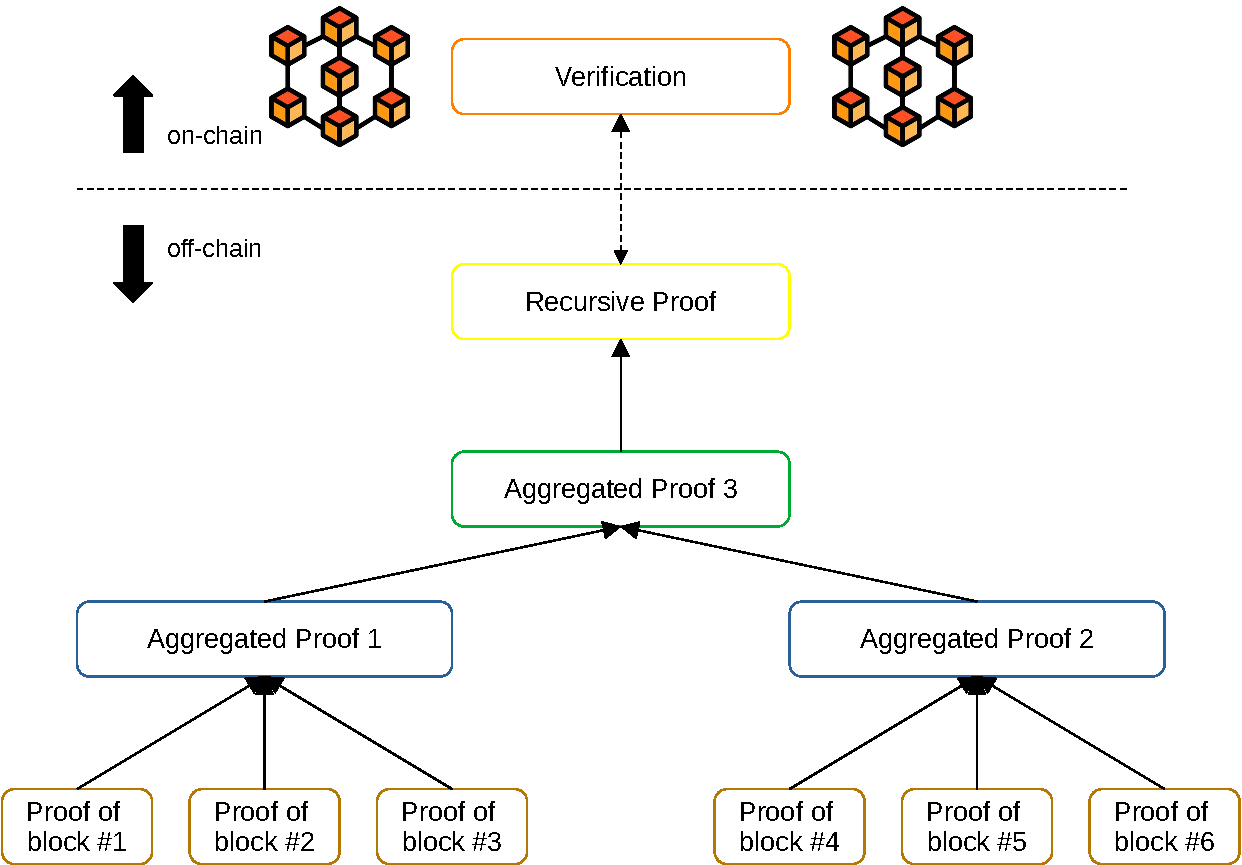
\includegraphics[width=.7\textwidth]{\recursiondir/figures/composition-blockchain}
	\caption{Design candidate's diagram of a proving scheme for the blockchain scalability issue.}
	\label{fig:composition-blockchain}
\end{figure}
As it can be observed, there is a trade-off between the number of blocks to aggregate and time required to perform such proofs. Finding the best scheme for off-chain proving is still an active area of research since there are many variables that come into the place. Which SNARKs to choose, how to combine them efficiently or how to organize the proof generalization are still open questions for those technologies building on top of thes ideas.

The prominent realization of this idea are \textit{rollups} \cite{Thibault2022}, \cite{Lavaur2022}. Section \ref{sec:scalability} will develop on the details about the core ideas of rollups.



%%%%%%%%%%%%%%%%%%%%%%%%%%%%%%%%%%%%%%%%%%%%%%%%%%%%%%%%%%%%%%%%%%%
\subsection{What about Zero-Knowledge?}

There is a good reason why zero-knowledge has not been discuseed up until this point in the whole section. The key fact is that the resulting composed SNARK satisfies the zero-knowledge property if and only if the last SNARK in the composition satisfies it. More exemplified, if $\B$ satisfies zero-knowledge, then so the composition of any other (and any number) SNARK with $\B$ as long as $\B$ is computed the last.

Hence, here we encounter a new potential benefit of proof composition: composing a highly efficient but not zero-knowledge SNARK $\A$ with a zero-knowledge SNARK $\B$ yields a zero-knowledge (and probably highly efficient) SNARK $\C = \B \circ \A$. 

\fi





%%%%%%%%%%%%%%%%%%%%%%%%%%%%%%%%%%%%%%%%%%%%%%%%%%%%%%%%%%%%%%%%%%%%%%%%%%%%%%%%
%TODO:¿¿ \subsubsection{Modular Design}



%%%%%%%%%%%%%%%%%%%%%%%%%%%%%%%%%%%%%%%%%%%%%%%%%%%%%%%%%%%%%%%
\section{Tools}

\subsection{PIL}

Polynomial Identity Language (PIL) is a novel domain-specific language to define the constraints of computation traces of either computations based on the circuit model or computations based on the state machine model. 
The constraints of the zkEVM execution trace, which is based on a state machine, are specified with PIL.


\subsection{Circom}

In Figure \ref{fig:circom_architecture} we show the architecture of Circom.
Programmers can use the Circom language to define arithmetic circuits and the compiler generates a file with the set of associated R1CS constraints together with a program (written either in cpp or wasm) that can be run to efficiently compute a valid assignment to all wires of the circuit.

After compiling a circuit, we can calculate all the signals that match the set of constraints of the circuit using the cpp or wasm programs generated by the compiler. To do so, we simply need to provide a file with a set of valid input values, and the program will calculate a set of values for the rest of signals of the circuit. A valid set of input, intermediate and output values is called \textit{witness}.

\begin{figure}[H]
\centering
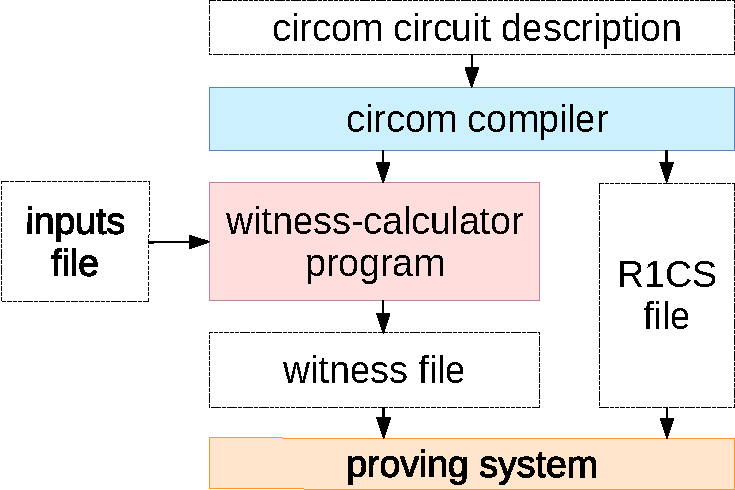
\includegraphics[width=0.5\textwidth]{\recursiondir/figures/circom-architecture}
\caption{Circom}
\label{fig:circom_architecture}
\end{figure}



\subsection{Non-recursive STARK \label{subsec:non_recursive_STARK}}

The setting for STARK proofs are machine-like computations from which we can derive a certain arithmetization, 
giving us a set of constraints describing its correct execution. 
The polynomial building the constraints that arise from a certain arithmetization can, 
in fact, depend on the inputs of the state machine itself giving what we call \textit{committed polynomials} and, 
by definition, should be computed once per proof. 
However, a polynomial that is completely independent of the input values so it is kept constant among several executions of the same state machine should be computed only once per arithmetization. 
The former kind of polynomials are called \textit{constant polynomials} and represent the computation that is being executed, so that they are publicly available for both the prover and the verifier, unlike the committed ones, which are not directly available to the verifier.


\begin{figure}[H]
\centering
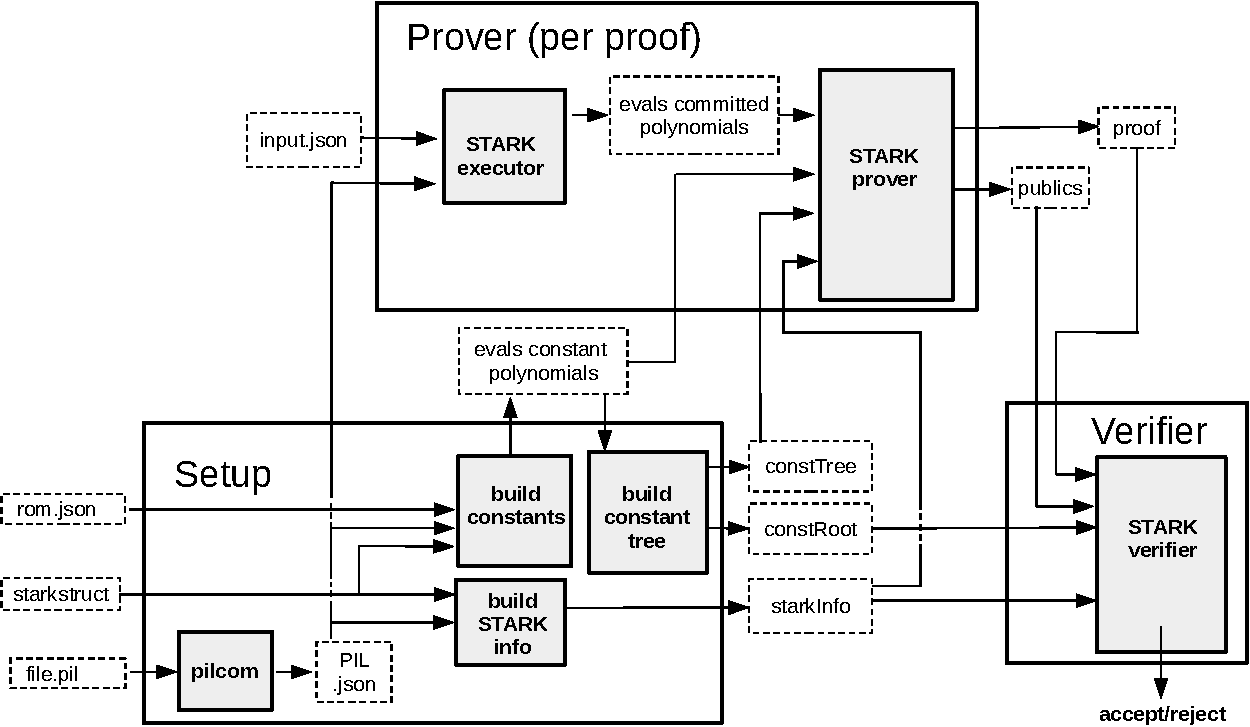
\includegraphics[width=\textwidth]{\recursiondir/figures/pil-stark-no_recursive-blocks}
\caption{Non recursive STARK.}
\label{fig:non-recursive}
\end{figure}

Due to the fact that all the constant polynomials do not depend on the particular inputs of a certain computation executed by the state machine, we can split the processes that make up the generation of a proof in two: the \textit{setup phase} and the \textit{proving phase}. 
This allows to execute both processes separately, which is highly important in order not to execute the constants' computation per proof, drastically increasing the proving time. 

The \textit{setup phase} performs all the pre-processing. 
The setup is only done once per state machine definition, allowing to reuse it whether the definition does not change. 
The definition of a state machine with \texttt{pil-stark} has three parts:

\begin{compactitem}
\item The \texttt{rom.json} file to build the computation.
\item The configuration of the FRI used in the STARK proof, inside a \texttt{starkstruct} file, specifying the blowup factor, the size of the trace and its LDE (Low Degree Extension) and the number of queries to be performed.
\item The \texttt{PIL} description of the STARK state machine, that is to say, the constraints that define the correctness of the execution trace (\texttt{file.pil} file).
\end{compactitem}

The PIL file and the \texttt{starkstruct} are used by the \texttt{build STARK info} process to write a file called \texttt{starkInfo} containing, apart from all the FRI-related parameters, several useful fields related with the PIL and the shape of the constraints. The PIL description is parsed with a compiler called \texttt{pilcom}\footnote{The \texttt{pilcom} parser is written with \url{https://github.com/zaach/jison}, which generates bottom-up parsers in JavaScript.} to obtain a parsed JSON version of the PIL, which will be used by the prover to compute all the polynomials involved in the proving procedure. The \texttt{build constants} process, using the parsed PIL, computes the evaluations of the constant polynomials over the evaluation domain determined by the \texttt{starkstruct}. Additionally, once this evaluations are computed, the \texttt{build constant tree} process generates the Merkle root of its corresponding tree for the verifier, which we call constant root (\texttt{constRoot}). 

In the \textit{proving phase}, the Prover executes all the processes that, given an input, generate a proof for the computation. 
The STARK executor process computes the evaluations of the polynomials that are going to be committed. To do so, it takes the names and descriptions of the polynomials from the parsed PIL and the provided inputs. Observe that, since the values of the committed polynomials are strongly dependent on the inputs, this procedure should be executed once per proof, unlike the setup phase. 

Finally, the \texttt{pil-stark} STARK prover process takes the evaluations of both the constant and the committed polynomials of the previous steps and all the information stored in the \texttt{starkInfo} object in order to generate the corresponding STARK proof and the associated public values for which the proof is valid. 
We use the \textsf{eSTARK} protocol, which is specially designed to proof PIL statements. 
The \textsf{eSTARK} protocol is composed on two main stages:

\begin{itemize}
\item \textit{Low-Degree Reduction phase}: Following \cite{EPRINT:StarkWare21}, first of all, we obtain a polynomial called FRI which codifies the validity of the values of the trace according to the PIL into the fact that it has low degree. This polynomial is committed to the verifier, as well as several previous polynomials that are used to provide consistency checks between them.  This phase, however, differs from the one described in \cite{EPRINT:StarkWare21} because PIL also accepts, apart from polynomial equalities, arguments such lookups, permutations or even copy-constraints (called connection arguments). Hence, this phase needs to be adapted in order to proof the correctness of each of the enumerated arguments. This serves as a motivation to call this protocol \textsf{eSTARK}, standing for \textit{extended STARK}. 

\item \textit{FRI phase}: After obtaining the so called FRI polynomial, the prover and the verifier are involved into a FRI Protocol \cite{ICALP:BBHR18}, aiming for proving that the committed polynomial has low degree (more concretely, it proves that the committed values of the polynomials raise a function that is close enough to a polynomial of low degree, see \cite{ICALP:BBHR18} for more information on FRI Protocol). 
\end{itemize}

The first stage can, in turn, be divided into several rounds. Below, we describe in a high level what is each of the rounds aiming.

\begin{itemize}

\item \textit{Round 1:} Given the trace column polynomials interpolating the execution trace, the prover commits to them.

\item \textit{Round 2:} The prover commits, for each lookup argument, to the $h$-polynomials of the modified \plookup version described in \cite{EPRINT:PFMBM22} (see \cite{EPRINT:GabWil20} for more information about \plookup protocol).

\item \textit{Round 3:} The prover commits to the grand-product polynomials for each of the arguments appearing in the PIL together with some intermediate polynomials used to reduce the degree of the grand products. This is due to the fact that \texttt{pil-stark} imposes a degree bound when committing to a polynomial. See \cite{EPRINT:GabWilCio19, EPRINT:GabWil20} for the specification of the grand-products of each of the different arguments allowed in PIL.

\item \textit{Round 4:} The prover commits to the $2$ polynomials $Q_1, Q_2$ arising from the splitting of the quotient polynomial $Q$. 

\item \textit{Round 5:} The prover provides the verifier with all the necessary evaluations of the polynomials so that he/she can execute the corresponding checks. 

\item \textit{Round 6:} The prover receives two randomness from the verifier which are used to construct the previously described FRI polynomial. Then, the prover and the verifier are involved into a FRI Protocol, ending with the prover sending the corresponding FRI proof to the verifier. 

\end{itemize} 


After the proof is generated, it is sent to the Verifier instance so that he/she can start the verification procedure, after what will accept or reject the proof. 



%%%%%%%%%%%%%%%%%%%%%%%%%%%%%%%%%%%%%%%%%%%%%%%%%%%%%%%%%%%%%%%
\section{Composition, Recursion and Aggregation}

\subsection{Composition}

As shown in Section \ref{subsec:non_recursive_STARK}, the basic verification of a STARK is performed by a verifier entity using the proof, the publics and some other verifier parameters.
Composing proofs means using different proving systems together to generate a proof.
Generally composition is used to increase the efficiency of some part of the system.
In our case, as first proving system we use a STARK and our main idea of composition is to delegate the verification procedure of the STARK proof $\pi_{STARK}$ to a verification circuit $C$.
In this case, if the prover provides a proof for the correct execution of the verification circuit $\pi_{CIRCUIT}$, then this is enough to verify the original STARK.
As shown in Figure \ref{fig:simple-composition}, in this case, 
the verifier entity just verifies the proof of the STARK verification circuit $\pi_{CIRCUIT}$.
The advantage of this composition is that $\pi_{CIRCUIT}$ is smaller and faster to verify than $\pi_{STARK}$.

\begin{figure}[H]
\centering
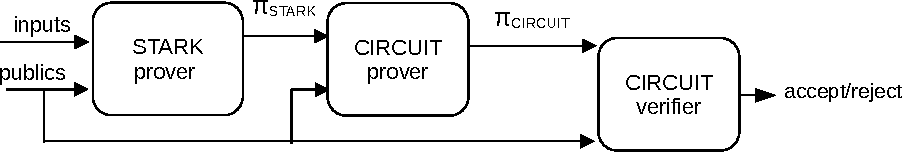
\includegraphics[width=0.7\textwidth]{\recursiondir/figures/simple-composition}
\caption{Simple composition.}
\label{fig:simple-composition}
\end{figure}

\subsection{Recursion}

\subsubsection{Setup Phase}

Since verifiers are much more efficient than provers, we can use this fact to create a recursive cascade of verifiers in which at each step we achieve a proof that can be more efficiently verified.
In our architecture, we create a chain of STARK verifiers using intermediate circuits for the definition of these STARK verifiers as shown in Figure \ref{fig:recursion-setup}.
We use circuits because they are suitable for computations with limited branching and a verifier is a computation of this type.

\begin{figure}[H]
\centering
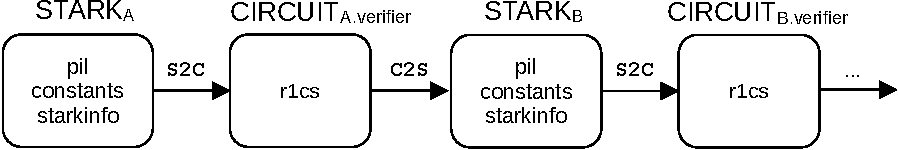
\includegraphics[width=0.8\textwidth]{\recursiondir/figures/recursion-setup}
\caption{Recursion setup.}
\label{fig:recursion-setup}
\end{figure}

Following Figure \ref{fig:recursion-setup}, lets consider that 
we have the parameters that describe the first STARK (pil, constants and starkinfo).
This first STARK that we denote as $\texttt{STARK}_{\texttt{A}}$, is then automatically translated into its verifier circuit. 
The STARK verifier circuit is described with R1CS constraints.
This translation, that we call \stoc (STARK-to-CIRCUIT), is performed in a setup phase. In other words, the R1CS description of the STARK verifier circuit can be pre-processed before the computation of the proof. 
We use Circom as intermediate representation language for the description of the circuits (see Section \ref{subsec:stoc} for more details about \stoc).

Next, we take the circuit definition (R1CS) and automatically translate it into a new STARK definition, that is to say, a new pil, new constants and a starkinfo.
This translation, that we call \ctos (CIRCUIT-to-STARK), 
is performed also in a setup phase.
Following our example, the new generated STARK is denoted as
$\texttt{STARK}_{\texttt{B}}$ and it is essentially a \plonk{ish} arithmetization with some custom gates of the verification circuit of $\texttt{STARK}_{\texttt{A}}$
(for more details about \stoc see Section \ref{subsec:ctos}).
It is worth to mention that these recursion steps can be applied as many times as desired taking into account that each step will compress the proof making it
more efficient to verify but increasing the prover complexity.
Finally, remark that during the setup phase, several artifacts for generating each STARK prover are generated (see Sections \ref{subsec:stoc} and \ref{subsec:ctos} for more information 
about these artifacts). 

\subsubsection{Proving Phase \label{subsubsec:proving:phase:intro}}


The first proof is generated by providing the proper inputs and public values to the first STARK prover. Then, the output proof is passed as input to the next STARK prover together with the public inputs and the process is recursively repeated.
In Figure \ref{fig:recursive-provers} we show how in essence a chain of recursive STARK provers work.

\begin{figure}[H]
\centering
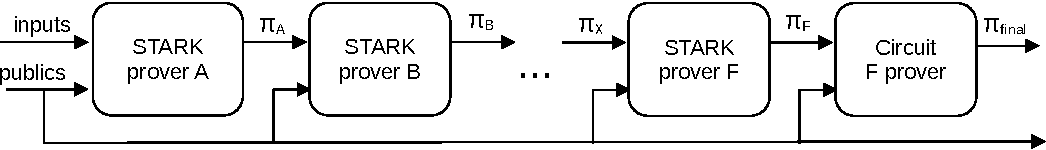
\includegraphics[width=0.95\textwidth]{\recursiondir/figures/recursive-provers}
\caption{Recursive provers.}
\label{fig:recursive-provers}
\end{figure}

Notice that the final proof is actually a circuit-based proof (currently we are using a Groth16 proof). More details about the proving phase can be found in Section \ref{subsec:recursion:step:proof}.


\subsection{Aggregation} 

Our architecture also allows aggregation when generating the proofs. Aggregation is a particular type of proof composition in which multiple valid proofs can be all proven to be valid by comprising them all into one proof, called the \textit{aggregated proof}, and only validating the aggregated one.
In our architecture, aggregators are defined in intermediate circuits.
Figure \ref{fig:aggregation_example} shows an example of aggregation with binary aggregators.
\begin{figure}[H]
\centering
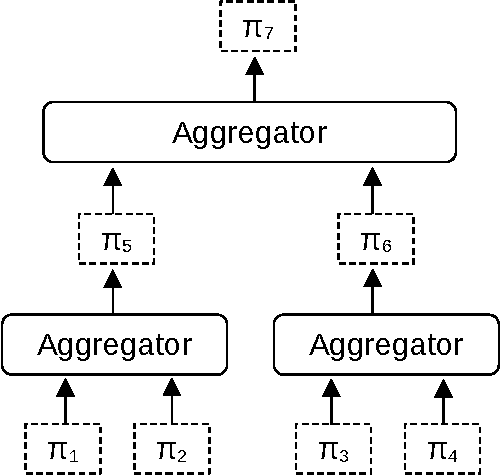
\includegraphics[width=0.4\textwidth]{\recursiondir/figures/radix-2-aggregation}
\caption{Aggregation example.}
\label{fig:aggregation_example}
\end{figure}


\subsection{Setup \stoc \label{subsec:stoc}}

Recall that we denote \stoc to the process of converting a given STARK into its verifier circuit, which is described in Circom and compiled to the corresponding R1CS constraints. The architecture of this generic conversion is depicted in Figure \ref{fig:setup-p2c}, where a \texttt{STARK}$_\texttt{x}$ is converted into a circuit denoted as $C_y$.


\begin{figure}[H]
\centering
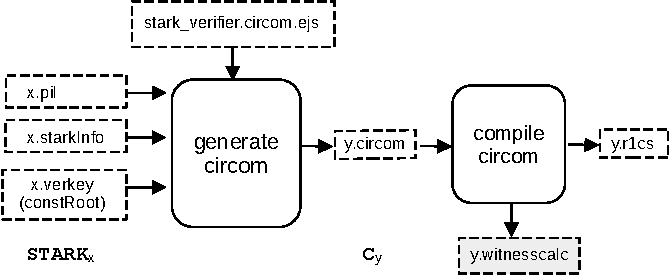
\includegraphics[width=0.8\textwidth]{\recursiondir/figures/setup-s2c}
\caption{Setup \stoc.}
\label{fig:setup-p2c}
\end{figure}

The input of the \stoc step is all the information needed to set up a circuit verifying the given STARK. 
In our architecture this is a PIL file specifying the STARK constraints that are going to be validated and the polynomial names, a \texttt{starkInfo} file containing the FRI-related parameters (blowup factor, the number of queries to be done, etc.), 
and the Merkle tree root of the computation constants (\texttt{constRoot}).
The output of the generate Circom process is a Circom description. 
The circuit is actually generated by filling an  \texttt{EJS} template
for the Circom description using the constraints defined by the PIL, the FRI-related parameters included by the \texttt{starkInfo} file and the \texttt{constRoot}. 
As shown in Figure \ref{fig:stark-verifier-circuit}, the inputs of the generated STARK verifier circuits are divided in two groups: the public inputs and the private inputs.

\begin{figure}[H]
\centering
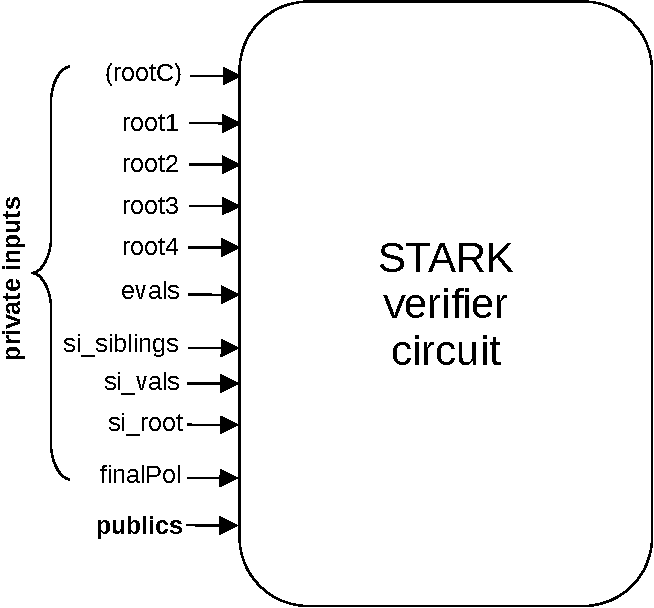
\includegraphics[width=0.55\textwidth]{\recursiondir/figures/STARK-verifier-inputs}
\caption{Inputs of the STARK verifier circuits.}
\label{fig:stark-verifier-circuit}
\end{figure}

The private inputs are the parameters of the previous STARK proof:

%TODO: Marc -> All: Enable should be reviewed
%TODO: Jose -> All: review description with info from Roger

\begin{itemize}

\item \texttt{(rootC)}: Four field elements being the root of the Merkle tree for the evaluations of constant (that is, preprocessed) polynomials of the previous STARK.
In some of the intermediate circuits that we generate, \texttt{rootC} is an input of the circuit while in other generated circuits \texttt{rootC} are internal signals 
hardcoded to the corresponding values (more information for each particular case is provided later).

\item \texttt{root1}: Four field elements being the root of the Merkle tree for the evaluations of all the trace column polynomials for the execution trace. 

\item \texttt{root2}: Four field elements being the root of the Merkle tree for the evaluations of the $h$ polynomials appearing in each lookup argument of the previous STARK. This root may be $0$ if no lookup argument is provided in the PIL.  

\item \texttt{root3}: Four field elements being the root of the Merkle tree for the evaluations of the grand product polynomials appearing in each argument (that is, lookup, permutation or connection arguments) of the previous STARK and the intermediate polynomials appearing in certain splitting of them. This root may be $0$ if no arguments are provided in the PIL. 

\item \texttt{root4}: Four field elements being the root of the Merkle tree for the evaluations of the splitting $Q_1$ and $Q_2$ of the $Q$ polynomial of the previous STARK.

\item \texttt{evals}: Contains all the necessary evaluations for all the polynomials appearing in the FRI verification process at a challenge value $z$ and at $gz$. 

\item \texttt{si\_root}: Four field elements being their root of the Merkle tree for the evaluations of the $i$-folded FRI polynomial, that is, the polynomial appearing in the $i$-th step of the FRI verification. 

\item \texttt{si\_vals}: The leaves' values of the previous Merkle tree used to check all the queries. The total amount of such values depends on the number of queries and the reduction factor attached to the current step of the FRI. 


\item \texttt{si\_siblings}: Merkle proofs for each of the previous evaluations.

\item \texttt{finalPol}: Contains all the evaluations of the last step's folding polynomial constructed in the FRI verification procedure over the last defined domain which has the same size as the degree of the polynomial. 

\end{itemize}

The \texttt{publics} are a set of inputs that will be used by the verifier to check the final prove and also by the intermediate STARKs (more information about publics used in the zkEVM STARK is provided in Section \ref{subsec:zkEVM:architecture}).

The final process to complete the \stoc step is to compile the Circom description to obtain a file with the associated R1CS constraints and a witness calculator program capable of compute all the values of the circuit wires for a given set of inputs.

Finally, remark that the particular intermediate circuit generated in a \stoc step,  denoted as $C_y$ in Figure \ref{fig:setup-p2c}, can be just a verifier of the previous STARK (\texttt{STARK}$_\texttt{x}$ in Figure \ref{fig:setup-p2c}) if we are only applying a recursion step, but more generally, other types of circuits that include the verifier but provide more functionality can be used. 
This latter is the case when we use circuits to verify aggregation of proofs.


\subsection{Setup \ctos \label{subsec:ctos}}

In our proving architecture, we create a chain of STARKs. 
From the \stoc step we can obtain a circuit that has to be converted again 
into a STARK. 
The step that achieves this conversion is a pre-processing step 
that we call \ctos. A picture of a generic \ctos step can be found in Figure \ref{fig:setup-c2s}, where a circuit denoted as $C_y$
is converted into its corresponding STARK (\texttt{STARK}$_\texttt{y}$).

\begin{figure}[H]
\centering
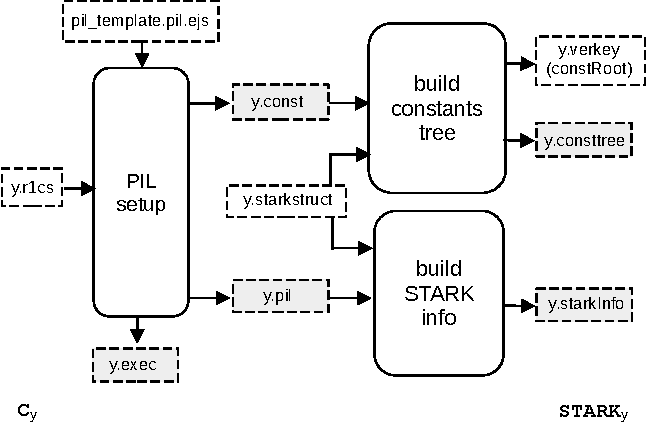
\includegraphics[width=0.75\textwidth]{\recursiondir/figures/setup-c2s}
\caption{Setup recursion step \ctos.}
\label{fig:setup-c2s}
\end{figure}

In more detail, the STARK arithmetization of the intermediate circuits of our proving architecture is a \plonk{ish} arithmetization with custom gates and using 12 polynomials for the values of the gate wires of the computation trace.
The STARK arithmetization includes several custom gates for doing specific tasks more efficiently. In particular, the custom gates provide the following functionality:

\begin{itemize}
\item \textbf{Poseidon}: This custom gate is capable of validating a Poseidon hash from a given $8$ field elements as inputs, $4$ field elements as capacity and a variable number of output elements. More specifically, this circuit implements the MDS matrix and the $7$-th power of field elements computations used to execute each of the rounds defined by the Poseidon hash sponge construction. 
\item \textbf{Extended Field Operations}: This custom gate is capable of validating multiplications and additions (or a combination of both) over the extended field $\FF_{p^3}$. The inputs are $3$ elements $a, b, c \in \FF_{p^3}$ and the output is corresponds to the element 
\[
a \cdot b + c \in \FF_{p^3}
\]
where the operations are defined over $\FF_{p^3}$. Observe that defining $c$ equal to $0$ one can compute pure multiplications. Similarly, setting $b$ equal to $1$, pure additions can be computed. 

\item \textbf{FFT}: This custom gate is in charge of computing FFT of a variable size in $\FF_p$ or in an extension field. 

\item \textbf{Polynomial Evaluation}: This custom gate is in charge of computing a single evaluation of polynomials in $\FF_{p^3}$ using Horner's rule. The input consists on a field element $z \in \FF_{p^3}$ and the coefficients of the polynomial $p$ which we are going to evaluate. The output is the evaluation $p(z) \in \FF_{p^3}$. 
\end{itemize}

We use selector polynomials to activate the custom gates of our STARK. 
These polynomials are constant (pre-processed). In particular, we use the selectors \texttt{POSEIDON12}, \texttt{GATE}, \texttt{CMULADD}, \texttt{EVPOL4} and \texttt{FFT4} are introduced. The selector \texttt{GATE} is actually in charge of activating a basic \plonk gate. The other selectors are in charge of selecting whichever subcircuit needs to be executed. Moreover, there also exist a special selector called \texttt{PARTIAL} which is in charge of distinguishing between partial and full layers in the Poseidon, since this affects the relationships between the values.

At this point we can detail the processes of the \ctos step.
As shown in Figure \ref{fig:setup-c2s}, the first process of the \ctos step is the PIL setup, which takes the R1CS constraints of a given intermediate circuit as input and produces all the STARK-related artifacts.
This includes the associated STARK identity constraints and the computation constants
that are respectively stored in a PIL file (\texttt{y.pil}) and in a file of constants
(\texttt{y.const}).
In particular, the identity constraints of the \plonk{ish} arithmetization are generated by filling an \texttt{EJS} template for the associated PIL (for the zkEVM the template used is called \texttt{compressor12.pil.ejs}). 

The PIL setup also generates an important file with exec extension (\texttt{y.exec})
that defines how to rearrange the values produced by the circuit witness calculator into the appropriate values of the STARK execution trace (see Thaler's book for more information about this rearrangement process). 
Notice that the rearrangement rules and the computation constants only depend on 
the circuit shape (which is coded in the \texttt{.r1cs} file generated by the Circom compiler). In other words, these parameters do not depend on the particular values of the circuit wires computed for a particular input.
Nevertheless, we will use the rearrangement rules file together with the witness values for a given input later on to build the STARK execution trace, which in turn is needed to generate the STARK proof.

Finally, we also produce the \texttt{starkInfo} file and a Merkle tree with the
STARK constants.

\subsection{Recursion Step Proof \label{subsec:recursion:step:proof}}

As we explained in Section \ref{subsubsec:proving:phase:intro}, to generate the final proof, we have to compute the proof of each 
intermediate STARK (see Figure \ref{fig:recursive-provers}).
Each intermediate STARK proof is generated using the witness values provided by the execution of the associated circuit witness computation program using as inputs the publics and the values of the previous proof.
Then, these values are properly rearranged to build the STARK execution trace using the corresponding \texttt{.exec} file.
In Figure \ref{fig:recursion:step:proof}, we provide the scheme of how the proof of an intermediate STARK is generated. 

\begin{figure}[H]
\centering
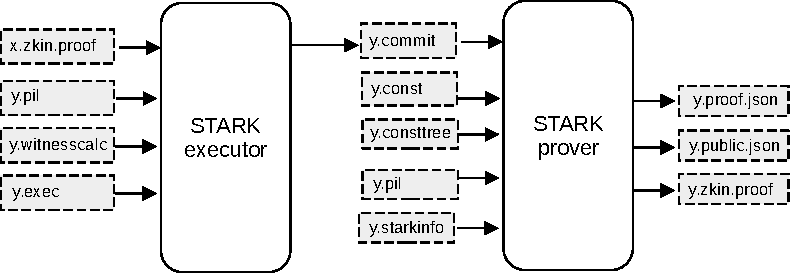
\includegraphics[width=0.9\textwidth]{\recursiondir/figures/recursive-step-proof}
\caption{STARK \texttt{Proof} of a recursion step.}
\label{fig:recursion:step:proof}
\end{figure}

As it can be observed, the STARK executor process takes the parameters of previous proof and the public inputs (both in the file \texttt{x.zkin.proof} which
has the proper format for the witness calculator generated by the Circom compiler), the PIL of the current STARK (\texttt{y.pil}), the witness calculator program of the associated circuit (\texttt{y.witnesscalc}) and the file of rearrangement rules (\texttt{y.exec}) to generate the non-preprocessed part of the STARK execution trace (\texttt{y.commit}). 
Next, the STARK prover process takes the execution trace, that is to say, the committed and constant polynomials, the constant tree, the corresponding PIL file and the information provided by the \texttt{zkevm.starkinfo.json} file to generate the proof.
Finally, when the proof is generated, the STARK prover process generates three files:

\vspace{0.1cm}
\begin{compactitem}
\item \textbf{Proof File} (\texttt{y.proof.json}): A json file containing the whole STARK proof in a \texttt{.json} file. 

\item \textbf{Publics File} (\texttt{y.public.json}): A json file containing only the publics. 

\item \textbf{zkIn File} (\texttt{y.zkin.proof.json}): A json file combining both the proof and the publics. 
\end{compactitem}


\section{Polygon zkEVM \label{section:polygon:zkevm}}

\subsection{Architecture \label{subsec:zkEVM:architecture}}

In this section, we provide the concrete blocks and steps used to
prove the correct execution of a batch of transactions (or several batches)
by our zkEVM using recursion, aggregation and composition.
As previously mentioned, generating a proof has two phases. 
The first phase is a setup executed only once per STARK computation definition. 
In our case, the STARK computation is the processing of batches by our zkEVM.  
In the setup phase, the different artifacts needed to generate proofs are preprocessed.
The second phase is when actually proofs are generated for given inputs (i.e. batches of transactions).
An overview of the overall process can be observed in figure \ref{fig:architecture-aggregation-recursion-composition}.

\begin{figure}[H]
\centering
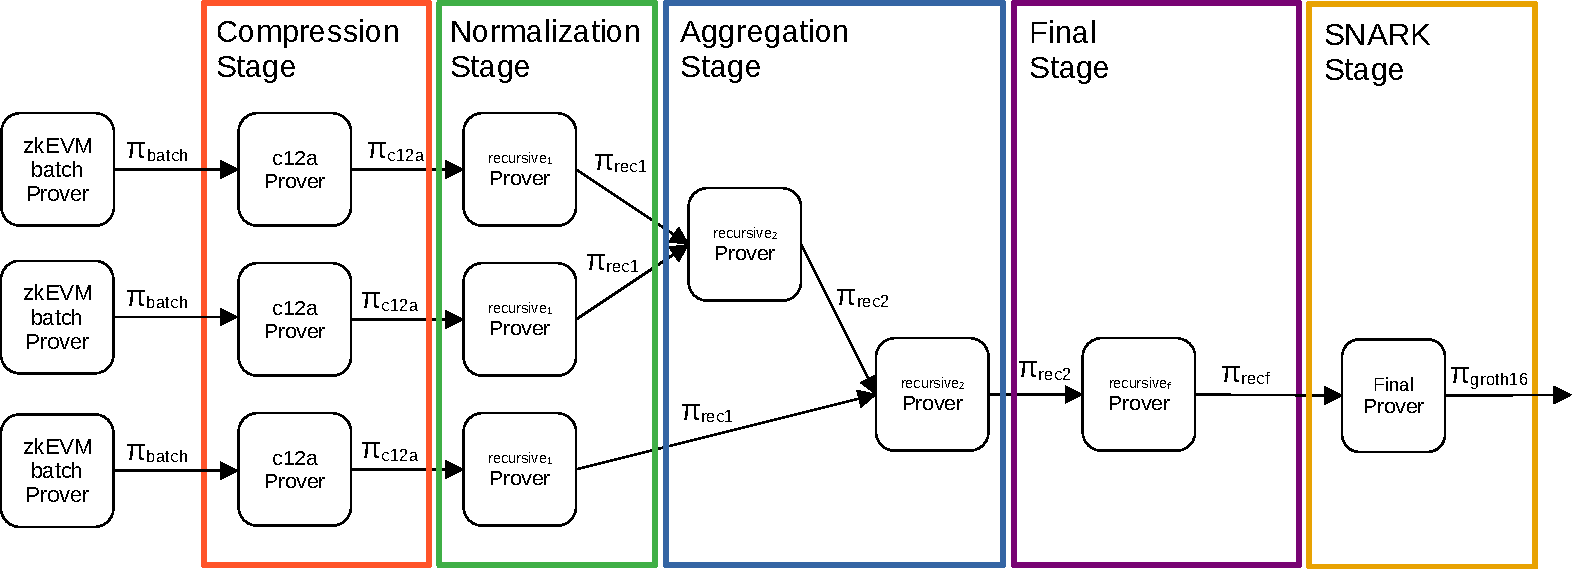
\includegraphics[width=\textwidth]{\recursiondir/figures/recursive-diagram-groth}
\caption{Proving architecture with recursion, aggregation and composition.}
\label{fig:architecture-aggregation-recursion-composition}
\end{figure}

Recall that the first STARK generates such a big proof since it has a lot of polynomials so its attached FRI uses a low blowup factor. Henceforth, a first \textit{Compression Stage} its invoked in each batch's proof, aiming to reduce the number of polynomials used, allowing to augment the blowup factor and therefore, reduce the proof size.  

Once the compression step has been completed, a proof aggregation stage will be in charge of joining several batches proofs into a single proof proving each of the single proofs all at once. The way of proceeding will be to construct a binary tree of proofs by aggregating two by two each of them. We will call this the \textit{Aggregation Stage}. 


However, since the aggregation of two proofs requires the constant root of the previous circuits through a public input coming from the previous circuit, there exists a \textit{Normalization Stage} which is in charge of transforming the obtained verifier circuit verifying the \texttt{c12a} proof into a one making the constant root public to the next circuit. This step allows each aggregator verifiers and the normalization verifiers to be exactly the same, permitting successful aggregation via a recursion. 

Once the normalization step has been finished, its time for aggregation. In this step we are going to join two batches' proofs together, which will be done many times until only one proof spares. In order to do so, a circuit capable of aggregating two verifiers is created. However, as we can see in the figure below, the inputs of this stage can be proofs of the kind $\pi_{\text{re1}}$ coming from the previous normalization stage, or  already aggregated proofs $\pi_{\text{re2}}$. This allows us to aggregate two $\pi_{\text{re1}}$ proofs, two $\pi_{\text{re2}}$ proofs or a combination of a $\pi_{\text{re1}}$ and a $\pi_{\text{re2}}$ proofs. Henceforth, this aggregation stage has to take into account this fact in its design. 


Observe that the \textit{Aggregation Stage} needs to be designed in order to accept either already aggregated proofs or only compressed ones. 
%\begin{figure}[H]
%\centering
%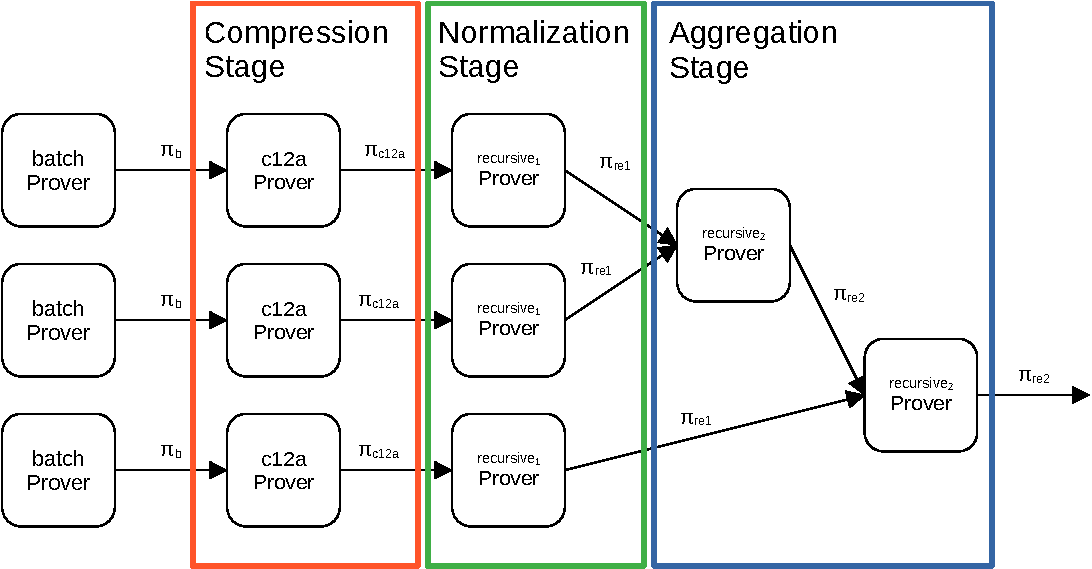
\includegraphics[width=\textwidth]{\recursiondir/figures/recursive-diagram-aggregation}
%\caption{Aggregation of proofs.}
%\label{fig:recursive-aggregation-intro}
%\end{figure}
The \textit{Final Stage} is the very last STARK step among the recursion process, which is in charge of verifying a $\pi_{\text{re2}}$ proof over a completely different finite field, the one defined by the \texttt{bn128} elliptic curve. More specifically, the hash in charge of generating the transcript will work over the field of the \texttt{bn128} curve. Hence, all the challenges (and so, all polynomials) will belong to this new field. This is done in this way because, in the next step of the process, a SNARK Groth16 proof, which works over elliptic curves, will be generated. In this step is very similar to the others, instantiating a verifier circuit for $\pi_{\text{re2}}$ but, in this case, $2$ constants roots should be provided (one for each of the proofs aggregated in the former step). 


%\begin{figure}[H]
%\centering
%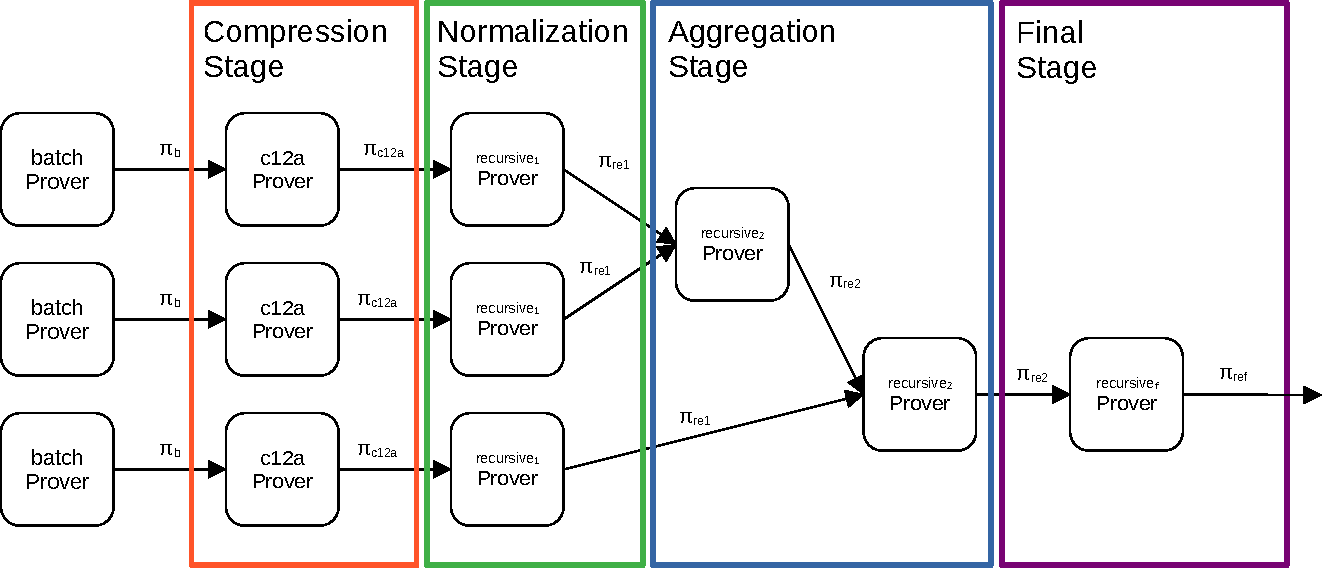
\includegraphics[width=\textwidth]{\recursiondir/figures/recursive-diagram-final}
%\caption{Final stage of the recursion.}
%\label{fig:recursivef-stage}
%\end{figure}

The last step of the whole process is called \textit{SNARK Stage}, and it purpose is to produce a Groth16 proof $\pi_{\text{groth16}}$ verifying the previous $\pi_{\text{ref}}$ proof. In fact, Groth16 can be replaced with any other SNARK proof. A SNARK is chosen here in order to reduce both verification complexity and proof size, which have constant complexity unlike STARK proofs. The $\pi_{\text{groth16}}$ proof will be sent to the verifier so that he/she can verify it. 


As a final remark, one should observe that the whole set of public inputs are being passed as inputs in each proof of the whole recursion procedure. The set of all public inputs is listed below (see the technical documents about the zkEVM L2 state management and the bridge):

\vspace{0.15cm}
\begin{compactitem}

\item \texttt{oldStateRoot}

\item \texttt{oldAccInputHash}

\item \texttt{oldBatchNum}

\item \texttt{chainId}

\item \texttt{midStateRoot}

\item \texttt{midAccInputHash}

\item \texttt{midBatchNum}

\item \texttt{newStateRoot}

\item \texttt{newAccInputHash}

\item \texttt{localExitRoot}

\item \texttt{newBatchNum}
\end{compactitem}

Next, let's describe the details of the steps and processes performed in each phase.

%%%%%%%%%%%%%%%%%%%%%%%%%%%%%%%%%%%%%%%%%%%%%%%%%%%%%%%%%
\subsection{Setup Phase}

The setup phase is a pre-processing phase in which all the artifacts for generating proofs are created. This includes the generation of intermediate circuits, which 
are a finite set of circuits that allow arbitrary combinations of proof recursions and proof aggregations.


%%%%%%%%%%%%%%%%%%%%%%%%%%%%%%%%%%%%%%%%%%%%%%%%%%%%%%%%%
\subsubsection{Build the zkEVM STARK}

As shown in Figure \ref{fig:zkevm:build}, we start by building the ROM of the zkEVM state machine, which is the program containing the instructions for the the executor that will generate the execution trace of the zkEVM. We also build the PIL that validates the execution trace. The ROM will, in fact, generate all the constant values for the execution trace of the zkEVM. Observe that, as said before, committed polynomials are not needed in the setup phase, so we need not run the executor of the zkEVM in order to generate them at this point. 

%TODO mirar que parte del starkInfo hace falta para generar el circom.

\begin{figure}[H]
\centering
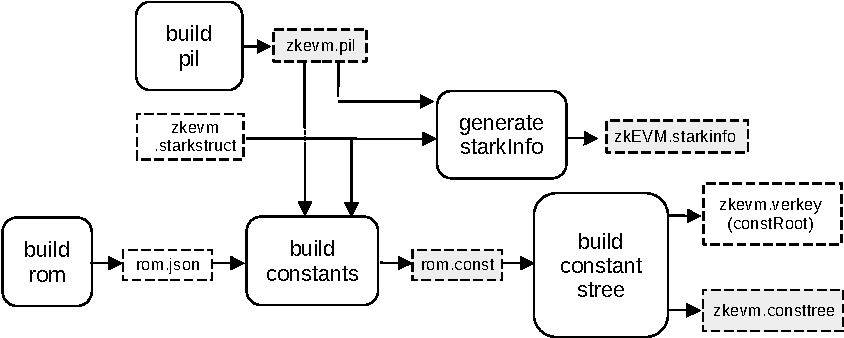
\includegraphics[width=0.85\textwidth]{\recursiondir/figures/zkevm-build}
\caption{Build the zkEVM STARK}
\label{fig:zkevm:build}
\end{figure}

The Merkle root of the tree of constant polynomials' evaluations, which is a hash that serves as cryptographic summary to capture all the fixed parameters of the computation, is stored as a parameter in a file called \texttt{zkevm.verkey}.
The last piece of data that is generated before building the STARK is the \texttt{starkInfo} that is necessary for automatically generating the circuit that will verify the zkEVM STARK. 
In this case, we use a blowup factor of $2$ and $128$ queries to generate the proof. 
The artifacts marked in gray will be used when generating the proof (proof generation is described in more detail in Section \ref{subsec:proof:gen:phase}). 





%%%%%%%%%%%%%%%%%%%%%%%%%%%%%%%%%%%%%%%%%%%%%%%%%%%%%%%%%
\subsubsection{Setup \stoc for the zkEVM STARK}

The next step in the setup is to generate the circuit to verify the zkEVM STARK (see Figure \ref{fig:zkevm:s2c}). 

\begin{figure}[H]
\centering
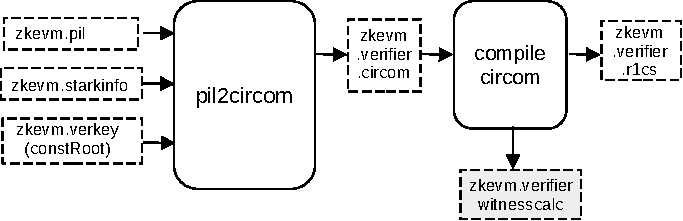
\includegraphics[width=0.8\textwidth]{\recursiondir/figures/zkevm-s2c}
\caption{Converting the zkEVM STARK verification into a circuit.}
\label{fig:zkevm:s2c}
\end{figure}


The \texttt{pil2circom} process fills an \texttt{EJS} template called \texttt{stark\_verifier.circom.ejs} with all the necessary information needed to validate the zkEVM STARK. Henceforth, we need to add the \texttt{zkevm.pil} in order to capture polynomial names, the \texttt{zkevm.starkinfo} file which specifies the blowup factor, the number of queries and the steps of the FRI-verification procedure and the \texttt{constRoot} in the \texttt{zkevm.verkey} file to automatically generates a circuit in Circom. The output Circom file \texttt{zkevm.verifier.circom} is then compiled into R1CS constraint system written in a file called \texttt{zkevm.verifier.r1cs}. This constraints will be used in the next step to generate the PIL and the constant polynomials for the next proof. 

On the other hand, the Circom compilation also outputs a witness calculator program that we call \texttt{zkevm.verifier.witnesscalc}. As it can be observed in the picture, the witness calculator program is marked in gray because it is going to be used when generating the proof.

Since our aim at the next proof generation will be compression (that is, proof size reduction) we will use a blowup factor of $4$ in this step, with $64$ queries. This information is contained in the \texttt{c12a.starkstruct} file located in the \texttt{proverjs} repository.



%%%%%%%%%%%%%%%%%%%%%%%%%%%%%%%%%%%%%%%%%%%%%%%%%%%%%%%%%
\subsubsection{Setup \ctos \texttt{c12a}}

The circuit that verifies the zkEVM STARK is called \texttt{zkevm.verifier} (or also \texttt{c12a}). This is because the PIL that is going to verify the \texttt{c12a} circuit is a \plonk{ish} circuit with custom gates and 12 polynomials aiming at compression. 

\begin{figure}[H]
\centering
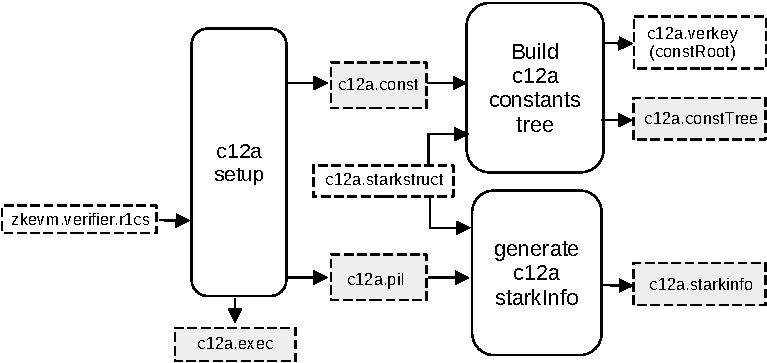
\includegraphics[width=0.85\textwidth]{\recursiondir/figures/c12a-c2s}
\caption{Convert the zkEVM verifier circuit to a STARK called \texttt{c12a}.}
\label{fig:zkevm-verifier-c2s}
\end{figure}

From the previous R1CS description of the verification circuit we are going to obtain a machine-like construction whose correct execution, which will be described by a PIL file, will be equivalent to the validity of the previous circuit. This process is started through a service called \texttt{compressor12\_setup}, where the corresponding PIL file for verifying the trace is output, as well as a binary for all the constant polynomials \texttt{c12a.const} defined by it. Moreover, a helper file called \texttt{c12a.exec} is generated by the same service. This helper file will contain all the necessary rules that will allow us to shuffle all the witness values, which will be computed later on, into the corresponding position of the execution trace. The design of this shuffling, together with the the connections defined in the constants polynomials \texttt{c12a.const} will ensure that, for a honest prover, this newly generated trace is valid whenever the previous circuit is. 

In order to finish the set up phase, having all the FRI-related parameters willing to be used in this step stored in a \texttt{c12a.starkstruct} file (located in the prover repository), we can generate the \texttt{c12a.starkinfo} file through the \texttt{generate\_starkinfo} service and build the constants' tree (and its respectively constant root). 




\subsubsection{Setup \stoc for \texttt{recursive1}}

Up to this point we have a STARK proof $\pi_{\text{c12a}}$ verifying the first big STARK proof $\pi$. The idea now is, as before, generate a Circom circuit that verifies $\pi_{\text{c12a}}$ by miming the FRI verification procedure. To do that, we generate a verifier circuit \texttt{c12a.verifier.circom} from the previously obtained \texttt{c12a.pil} file, the \texttt{c12a.starkinfo} file and the constant root \texttt{c12a.verkey.constRoot} by filling the \texttt{stark\_verifier.circom.ejs} template as before.

In this case, in seek of normalization, we need to briefly modify this circuit in order to include the constant root as a public input. Observe that, since we are not still aggregating, the constant root will not be actually used here, though this will be extremely important in the aggregation stage, where all the constants for the computation, which depend on the previous circuit, need to be provided as public inputs. This is done by using \texttt{recursive1.circom} file and importing inside the previously generated \texttt{c12a.verifier.circom} circuit as a library. The verifier circuit is instantiated inside \texttt{recursive1.circom}, connecting all the necessary wires and including the constant root to the set of publics. 

The output circom file \texttt{recursive1.circom} it is compiled into a R1CS \texttt{recursive1.r1cs} file and a witness calculator program \texttt{recursive1.witnesscal} which will be both used later on in order to build and fill the next execution trace. 

\begin{figure}[H]
\centering
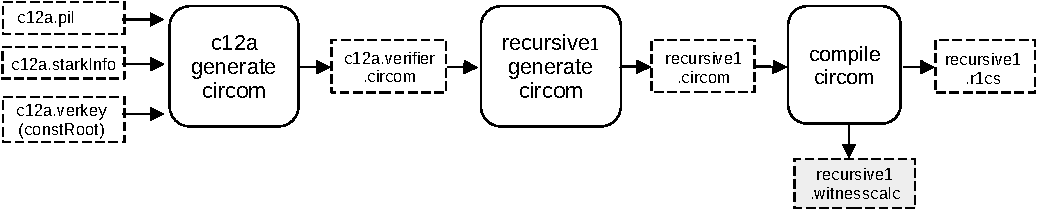
\includegraphics[width=\textwidth]{\recursiondir/figures/c12a-s2c}
\caption{Convert the c12a STARK to a c12a verifier circuit.}
\label{fig:c12a-s2c}
\end{figure}

\subsubsection{Setup \ctos for \texttt{recursive1}}

As before, from the previous R1CS description of the verification circuit we are going to obtain a machine-like construction whose correct execution, which will be described by a PIL \texttt{recursive1.pil} file, will be equivalent to the validity of the previous circuit. Also, a binary for all the constant polynomials \texttt{recursive1.const} defined by it and the helper file providing the witness values allocation into its corresponding position of the execution trace \texttt{recursive1.exec} are generated.

In order to finish the set up phase, having all the FRI-related parameters willing to be used in this step stored in a \texttt{recursive.starkstruct} file (located in the prover repository), we can generate the \texttt{recursive1.starkinfo} file through the \texttt{generate\_starkinfo} service and build the constants' tree (and its respectively constant root). In this case, we are using a blowup factor of $2^4 = 16$, allowing the number of queries to be $32$. 

\begin{figure}[H]
\centering
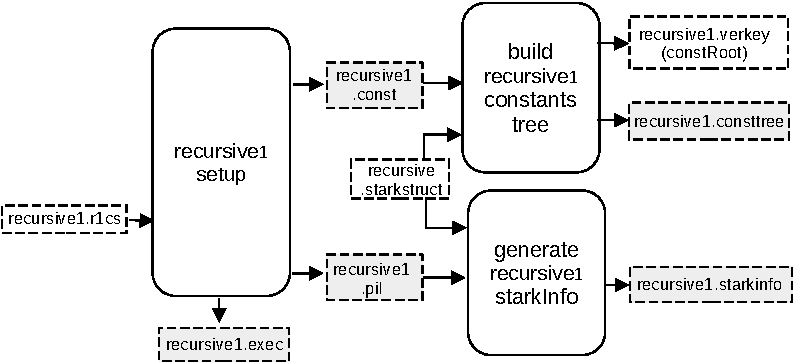
\includegraphics[width=.85\textwidth]{\recursiondir/figures/recursive1-c2s}
\caption{Convert the \texttt{recursive1} circuit to its associated STARK.}
\label{fig:recursive1-c2s}
\end{figure}



\subsubsection{Setup \stoc for \texttt{recursive2}}

Up to this point we have a STARK proof $\pi_{\text{re1}}$ verifying the proof $\pi_{\text{c12a}}$. As before, we generate a Circom circuit that verifies $\pi_{\text{re1}}$ by miming the FRI verification procedure. To do that, we generate a verifier circuit \texttt{recursive1.verifier.circom} from the previously obtained \texttt{recursive1.pil} file, the \texttt{recursive1.starkinfo} file and the constant root \texttt{recursive1.verkey.constRoot} by filling the verifier \texttt{stark\_verifier.circom.ejs} template.

After the verifier is generated using the template, we will also use a template to create another Circom that aggregates two verifiers. Note that, in the previous step, the constant root is passed harcoded into the circuit from an external file. But this was intended as a normalization, allowing the previous circuit and each ones verifying each of both proofs to have exactly the same form, allowing recursion being possible. Henceforth, this \texttt{recursive2.circom} circuit has two verifiers and a two multiplexors that are actually deciding the form of each of the verifiers: if the proof has $\pi_{\text{re1}}$ form, the hardcoded constant root is input but, if the proof has $\pi_{\text{re2}}$ form, the constant root should be connected as input signal, coming from a previous circuit. 

A schema of the \texttt{recursive2} circuit generated is as shown in Figure \ref{fig:recursive2-circuit}. Observe that, since the upper proof has the $\pi_{\text{re2}}$ form, the Multiplexor does not provides the constant root \texttt{rootC} to the Verifier A to hardcode it because this verifier should get it trough a public input from the previous circuit. Otherwise, the lower proof has the $\pi_{\text{re1}}$ form, so the Multiplexor let is pass trough the constant root into the Verifier B so that it can be hardcoded it when the corresponding template is filled. 

\begin{figure}[H]
	\centering
	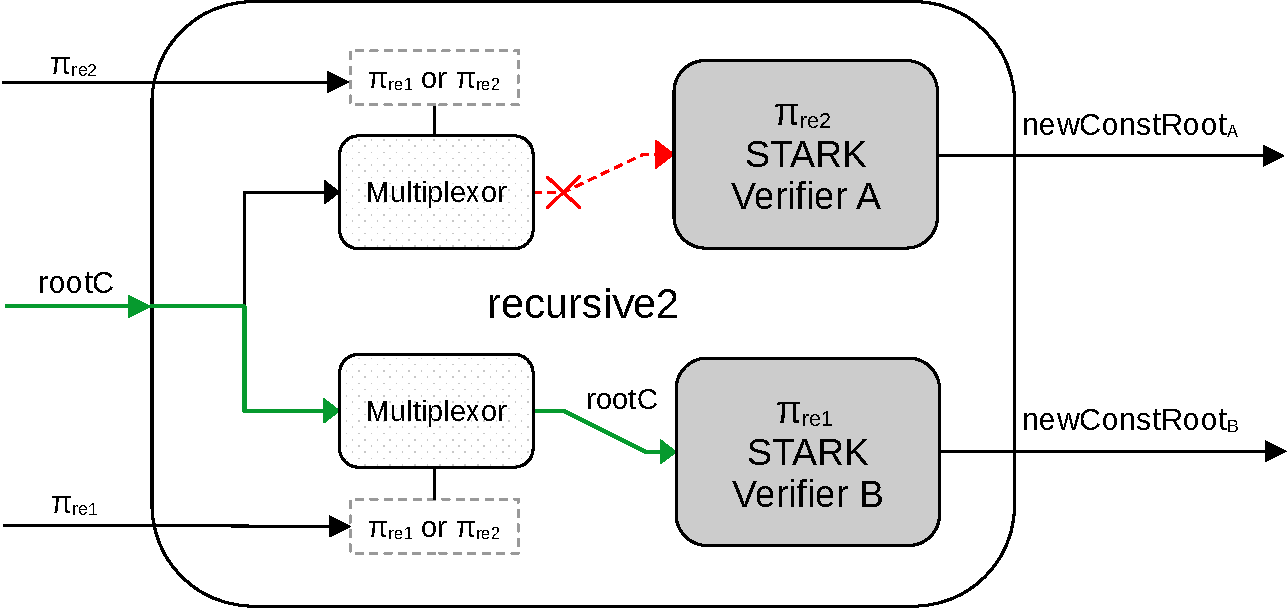
\includegraphics[width=0.9\textwidth]{\recursiondir/figures/recursive2-circuit}
	\caption{\texttt{recursive2} circuit.}
	\label{fig:recursive2-circuit}
\end{figure}


The output circom file \texttt{recursive2.circom}, obtained running a different script called \texttt{genrecursive} it is compiled into a R1CS \texttt{recursive2.r1cs} file and a witness calculator program \texttt{recursive2.witnesscal} which will be both used later on in order to build and fill the next execution trace. 

\begin{figure}[H]
\centering
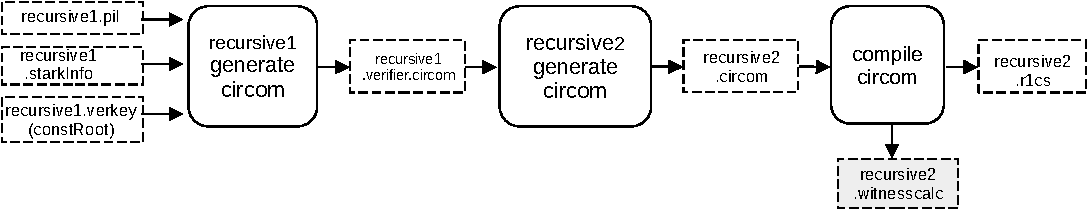
\includegraphics[width=\textwidth]{\recursiondir/figures/recursive1-s2c}
\caption{Convert the \texttt{recursive1} STARK to its verifier circuit called \texttt{recursive2}.}
\label{fig:recursive1-s2c}
\end{figure}




\subsubsection{Setup \ctos for \texttt{recursive2}}

As before, from the previous R1CS description of the verification circuit we are going to obtain a machine-like construction whose correct execution, which will be described by a PIL \texttt{recursive2.pil} file, will be equivalent to the validity of the previous circuit. Also, a binary for all the constant polynomials \texttt{recursive2.const} defined by it and the helper file providing the witness values allocation into its corresponding position of the execution trace \texttt{recursive2.exec} are generated.

In order to finish the set up phase, having all the FRI-related parameters willing to be used in this step stored in a \texttt{recursive.starkstruct} file (located in the prover repository), we can generate the \texttt{recursive2.starkinfo} file through the \texttt{generate\_starkinfo} service and build the constants' tree (and its respectively constant root). Since we want both verifiers to be exactly the same as in the previous step, we are using the same blowup factor of $2^4 = 16$, allowing the number of queries to be $32$. 

\begin{figure}[H]
	\centering
	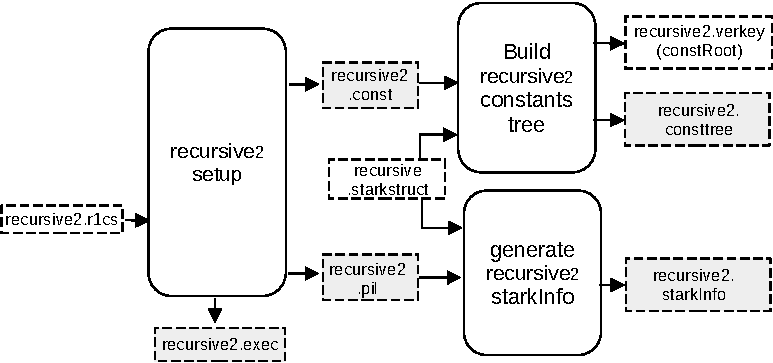
\includegraphics[width=.8\textwidth]{\recursiondir/figures/recursive2-c2s}
	\caption{Convert the \texttt{recursive2} circuit to its associated STARK.}
	\label{fig:recursive2-c2s}
\end{figure}



\subsubsection{Setup \stoc for \texttt{recursivef}}

Up to this point we have a STARK proof $\pi_{\text{re2}}$ verifying another  $\pi_{\text{re2}}$ proof (or $\pi_{\text{re1}}$ in some edge cases). The idea now is, as before, generate a Circom circuit that verifies $\pi_{\text{re2}}$ (or $\pi_{\text{re1}}$ if no aggregation is taking place) by miming the FRI verification procedure as done before. To do that, we generate a verifier circuit \texttt{recursive2.verifier.circom} from the previously obtained \texttt{recursive2.pil} file, the \texttt{recursive2.starkinfo} file and the constant roots of the previous two proofs \texttt{recursive2\_a.verkey.constRoot} and \texttt{recursive2\_b.verkey.constRoot} by filling the \texttt{stark\_verifier.circom.ejs} template as before.

The output circom file \texttt{recursivef.circom}, obtained running a different script called \texttt{genrecursivef} it is compiled into a R1CS \texttt{recursivef.r1cs} file and a witness calculator program \texttt{recursivef.witnesscal} which will be both used later on in order to build and fill the next execution trace. 

\begin{figure}[H]
\centering
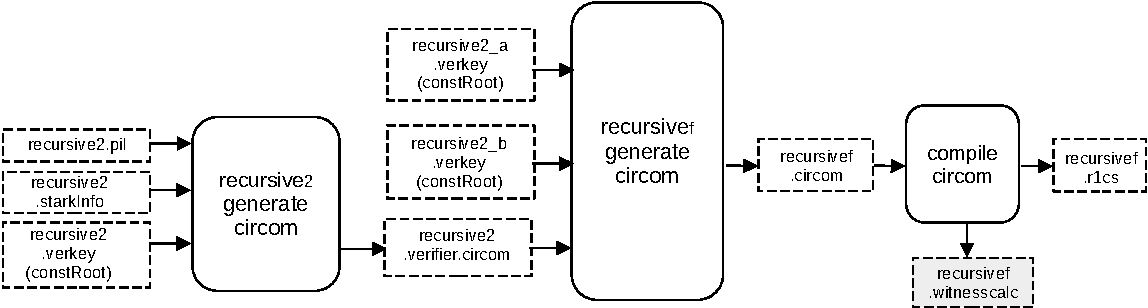
\includegraphics[width=\textwidth]{\recursiondir/figures/recursive2-s2c}
\caption{Convert the \texttt{recursive2} STARK to its verifier circuit called \texttt{recursivef}.}
\label{fig:recursive2-s2c}
\end{figure}

\subsubsection{Setup \ctos for \texttt{recursivef}}

As before, from the R1CS description of the verification circuit we are going to obtain a machine-like construction whose correct execution, which will be described by a \texttt{recursive2.pil} PIL file, will be equivalent to the validity of the previous circuit. Also, a binary for all the constant polynomials \texttt{recursive2.const} defined by it and the helper file providing the witness values allocation into its corresponding position of the execution trace \texttt{recursive2.exec} are generated.

In order to finish the set up phase, having all the FRI-related parameters willing to be used in this step stored in a \texttt{recursivef.starkstruct} file (located in the prover repository), we can generate the \texttt{recursivef.starkinfo} file through the \texttt{generate\_starkinfo} service and build the constants' tree (and its respectively constant root). 

\begin{figure}[H]
\centering
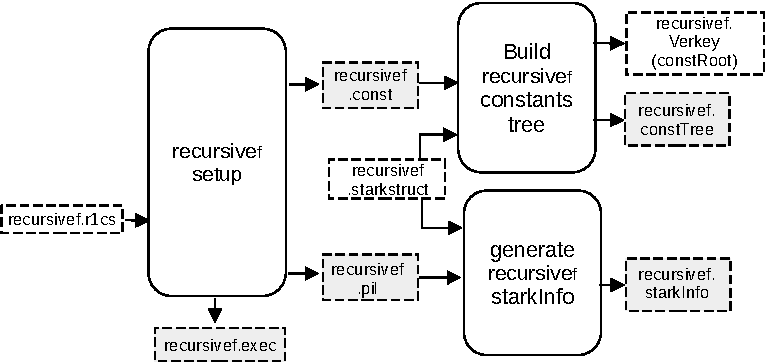
\includegraphics[width=0.8\textwidth]{\recursiondir/figures/recursivef-c2s}
\caption{Convert the recursivef circuit to its associated STARK.}
\label{fig:recursivef-c2s}
\end{figure}




\subsubsection{Setup \stoc for \texttt{final}}

Up to this point we have a STARK proof $\pi_{\text{ref}}$ verifying a proof $\pi_{\text{re2}}$. As before, we generate a Circom circuit that verifies $\pi_{\text{ref}}$ by miming the FRI verification procedure. To do that, we generate a verifier circuit \texttt{recursivef.verifier.circom} from the previously obtained \texttt{recursivef.pil} file, the \texttt{recursivef.starkinfo} file and the constant root \texttt{recursivef.verkey.constRoot} by filling the \texttt{stark\_verifier.circom.ejs} verifier template. This verifier Circom file will be imported by the \texttt{final.circom} circuit in order to generate the circuit that will be proven using Groth16 procedure. 



\begin{figure}[H]
	\centering
	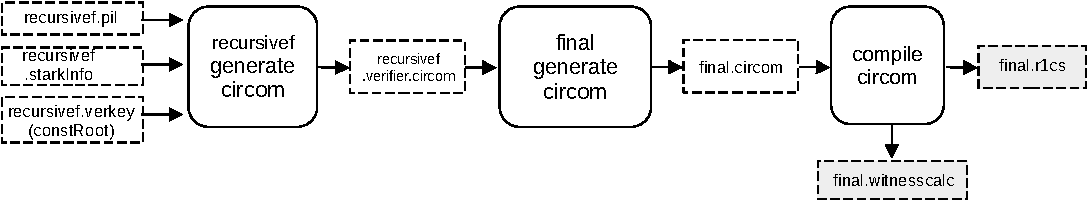
\includegraphics[width=\textwidth]{\recursiondir/figures/final-s2c}
	\caption{Convert the \texttt{recursivef} STARK to its verifier circuit that is called \texttt{final.circom}.}
	\label{fig:final-s2c}
\end{figure}



\subsection{Proof Generation Phase \label{subsec:proof:gen:phase}}

\subsubsection{Proof of the zkEVM STARK}

Up to this point we built an execution trace together with a PIL file describing the ROM of the zkEVM. Having both we can generate a STARK proof stating the correct execution of the zkEVM using the \texttt{pil-stark} tooling explained in section \ref{subsec:non_recursive_STARK}. In this step, a blowup factor of $2$ is used, so the proof having a huge amount of polynomials becomes quite big. To amend that, the next step \texttt{c12a} will be a compression step, raising the blowup factor and aiming to reduce the number of polynomials. 

\begin{figure}[H]
\centering
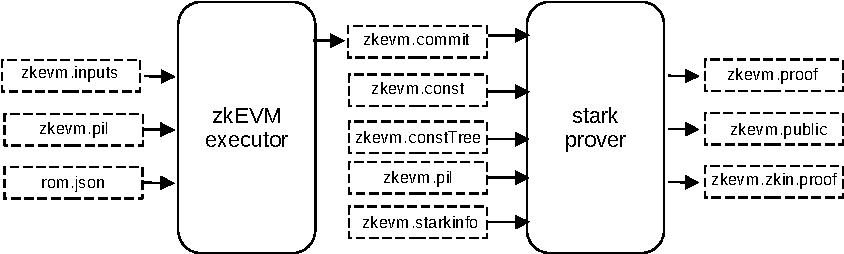
\includegraphics[width=0.85\textwidth]{\recursiondir/figures/zkevm-proof}
\caption{Generation for a zkEVM Proof}
\label{fig:recursive-zkemv-proof}
\end{figure}

To generate the proof, \texttt{main\_prover} service is used. The service requires to provide the execution trace (that is, the committed and constant polynomials files generated by the executor using the \texttt{pilcom} package), the constant tree binary file in order to be hashed to construct the constant root, the PIL file of the zkEVM ROM \texttt{zkev.pil} and all the information provided by the \texttt{zkevm.starkinfo.json} file, including all the FRI-related parameters such as the blowup factor or the configuration of the steps. 

This step differs from the next ones as it is the first and it is intended to start the recursion. However, aiming uniformization code-wise,  the Main Prover procedure choose to abstract the notion of proving and is intended to be the same at each step among the recursion. 



\subsubsection{Proof of \texttt{c12a}}


%TODO: Jose: The publics of c12a are the same as zkevm right?

To generate the proof verifying the previous \texttt{zkevm.proof}, we generate all the witness values and map them correctly into its corresponding position of the execution trace exactly in the same way as before, obtaining a binary file \texttt{ca12.commit} for the committed polynomials of the execution trace. 

Having the execution trace (that is, the committed and constant polynomials filled) and the PIL, we can generate a proof validating the previous big STARK proof. We use the same service \texttt{main\_prover} as before to do it, providing also the previously built constant tree \texttt{ca12.constTree} and the \texttt{ca12.starkinfo} file. This will generate the proof and the publics joined in the \texttt{c12a.zkin.proof} file.  

\begin{figure}[H]
\centering
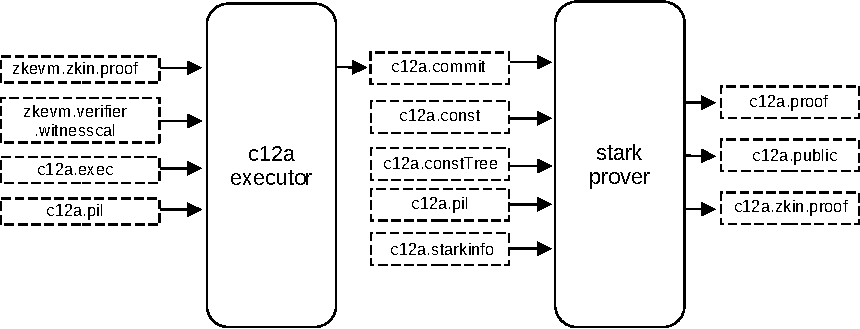
\includegraphics[width=0.77\textwidth]{\recursiondir/figures/c12a-proof}
\caption{Generate a STARK proof for \texttt{c12a}.}
\label{fig:c12a-proof}
\end{figure}



\subsubsection{Proof of \texttt{recursive1}}

To generate the proof verifying the previous \texttt{c12a.proof}, we generate all the witness values and map them correctly into its corresponding position of the execution trace exactly in the same way as before, obtaining a binary file \texttt{recursive1.commit} for the committed polynomials of the execution trace. 

Having the execution trace (that is, the committed and constant polynomials filled) and the PIL, we can generate a proof validating the previous big STARK proof. We use the same service \texttt{main\_prover} as before to do it, providing also the previously built constant tree \texttt{recursive1.constTree} and the \texttt{recursive1.starkinfo} file. This will generate the proof and the publics joined in the \texttt{recursive1.zkin.proof} file. 

\begin{figure}[H]
\centering
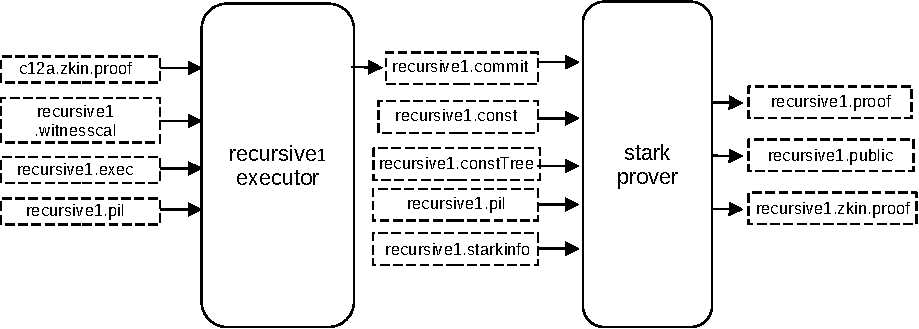
\includegraphics[width=0.85\textwidth]{\recursiondir/figures/recursive1-proof}
\caption{Generate a STARK proof for \texttt{recursive1}.}
\label{fig:recursive1-proof}
\end{figure}



\subsubsection{Proof of \texttt{recursive2}}

To generate the proof verifying the previous \texttt{recursive1.proof}, we generate all the witness values and map them correctly into its corresponding position of the execution trace exactly in the same way as before, obtaining a binary file \texttt{recursive2.commit} for the committed polynomials of the execution trace. 

Having the execution trace (that is, the committed and constant polynomials filled) and the PIL, we can generate a proof validating the previous big STARK proof. We use the same service \texttt{main\_prover} as before to do it, providing also the previously built constant tree \texttt{recursive2.constTree} and the \texttt{recursive2.starkinfo} file. This will generate the proof and the publics joined in the \texttt{recursive2.zkin.proof} file. 

\begin{figure}[H]
\centering
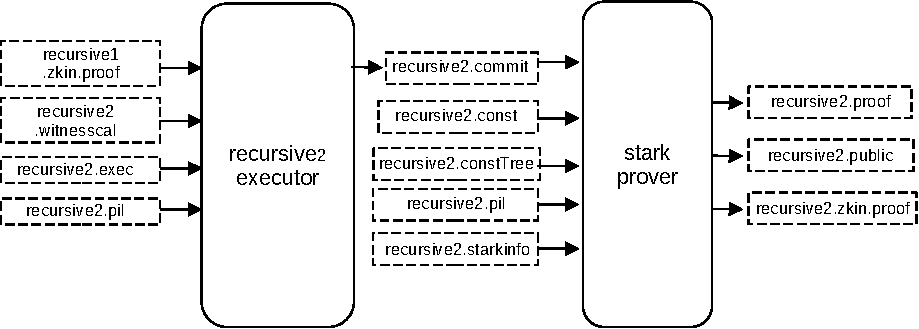
\includegraphics[width=\textwidth]{\recursiondir/figures/recursive2-proof}
\caption{Generate a STARK proof for \texttt{recursive2}.}
\label{fig:recursive2-proof}
\end{figure}


\subsubsection{Proof of \texttt{recursivef}}

To generate the proof verifying the previous \texttt{recursive2.proof}, we generate all the witness values and map them correctly into its corresponding position of the execution trace exactly in the same way as before, obtaining a binary file \texttt{recursivef.commit} for the committed polynomials of the execution trace. 

Having the execution trace (that is, the committed and constant polynomials filled) and the PIL, we can generate a proof validating the previous big STARK proof. We use the same service \texttt{main\_prover} as before to do it, providing also the previously built constant tree \texttt{recursivef.constTree} and the \texttt{recursivef.starkinfo} file. This will generate the proof and the publics joined in the \texttt{recursivef.zkin.proof} file. 


\begin{figure}[H]
\centering
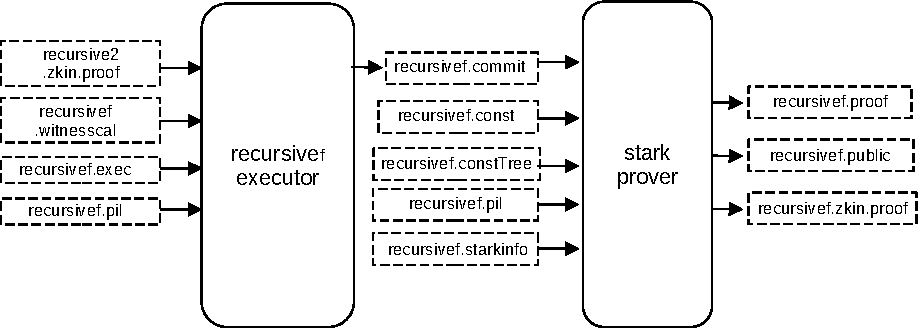
\includegraphics[width=0.77\textwidth]{\recursiondir/figures/recursivef-proof}
\caption{Generate a STARK proof for \texttt{recursivef}.}
\label{fig:recursivef-proof}
\end{figure}



\subsubsection{Proof of \texttt{final}}

The last circuit, \texttt{final.circom} is the one used to generate the proof.
At this moment a Groth16 proof is generated.


\section{Remarks}

The setup phase runs with the proverjs. The proof generation 
runs with the prover written in C.
The circuits build in the setup phase can be used as many times
as desired.
The prover receives the information about the particular composition of 
proofs with an RPC API.


%
%\subsection{Depth-One Composition ??}
%
%In order to achieve a composed proof system $\F = \O \circ \I$, we must take the verification procedure of $\I$ and feeding it through the proof machinery of $\O$. That is, a typical workflow would represent the verifier in $\I$ as an arithmetic circuit $C$ and then apply the prover in $\O$ to establish knowledge of a proof $\pi_{\I}$ such that $C(\pi_{\I}) = 1$. A high-level description can be seen in Figure \ref{fig:recursive-depth1}.
%
%There are two natural ways to obtain proof system composition by means of PIL and Circom:
%\begin{enumerate}
% \item[(a)] Use PIL to represent the verifier in $\I$ as a state machine $M$ such that $M(\pi_{\I}) = 1$ if and only if $\pi_{\I}$ is valid, and then use $\texttt{pil-stark}$ to generate a proof for $M$.
% \item[(b)] Use \texttt{pil2circom} to represent the verifier in $\I$ as an arithmetic circuit $C$ written in Circom such that $C(\pi_{\I}) = 1$ if and only if $\pi_{\I}$ is valid, then use $\texttt{r1cs2plonk}$ to transform the R1CS intermediate representation into PIL, and then use $\texttt{pil-stark}$ to generate a proof for the state machine of the last PIL. This process is depicted in Figure \ref{fig:recursive-depth1}.
%\end{enumerate}
%
%\begin{figure}[H]
%\centering
%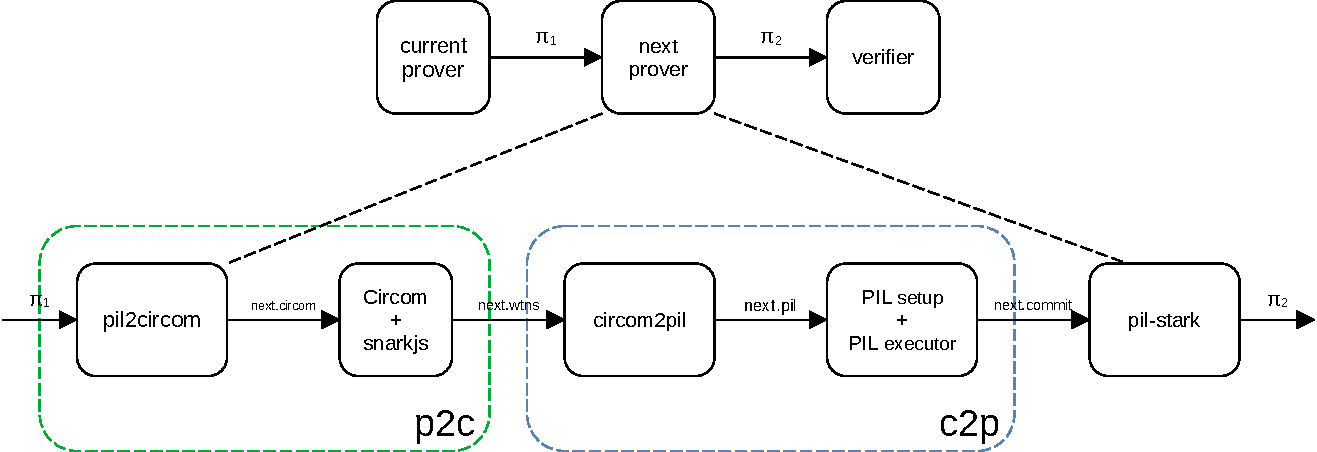
\includegraphics[width=\textwidth]{\recursiondir/figures/recursive-diagram-depth1}
%\caption{Depiction of a depth-one composition with focus on the workflow followed by the Prover to obtain the outer proof $\pi_{\O}$.}
%\label{fig:recursive-depth1}
%\end{figure}
%
%The Circom implementation of the inner STARK verification procedure can be found in \cite{HermezSTARKVerCircom2022}.